\documentclass{article}

\usepackage{graphicx}

\begin{document}

\title{Projecto de Algoritmos e Estruturas de dados}
\author{João Luís Freire Fraga, nº 39222}
\date{11 Janeiro 2019}

\clearpage\maketitle
\thispagestyle{empty}
\newpage

\section{Abordagem ao problema}

Comecei por ler o enunciado do problema e tentar perceber e interiorizar o que era pedido. Analisei brevemente os exemplos de input, a forma em que o output era esperado e, quando me senti confortável com o objetivo do projeto, decidi começar a pensar quais seriam os principais problemas com que me depararia durante a resolução do projeto.

Cheguei a conclusão que o meu trabalho estaria então, provavelmente, dividido em 2 grandes partes: Primeiro, teria de decidir quais as estruturas de dados a utilizar, tendo em conta o tamanho do input e a forma como futuramente chegaria a solução. Segundo, teria que pensar num algoritmo (e estruturas de dados associadas) que me permitisse, da forma o mais eficiente que me conseguisse lembrar, rapidamente descobrir regiões de pixéis dentro do intervalo de tolerância pedido.

\section{Armazenamento do input}

Uma vez que o nosso input se tratava de um vídeo, e um vídeo não é mais que uma sequência de “frames” compostos, por sua vez, por um conjunto de pixéis achei que provavelmente seria conveniente representar algumas destas entidades no meu programa e decidi então começar por criar 2 estruturas: Frame (Uma das muitas imagens do vídeo); Pixel (Conjunto de informações sobre um dos muitos pixéis do frame).

No enunciado do problema não foram fornecidas informações sobre a duração ou resolução máxima do vídeo, por isso decidi que iria representar o meu vídeo na forma de uma lista de frames (uma vez que não seria garantido conseguir alocar espaço continuo em memória suficiente para representar o vídeo inteiro sobre a forma de um array); Decidi também que cada frame iria conter um array de arrays de apontadores para pixéis.

Ao longo da resolução do projeto, acabei por implementar outras estruturas de dados e adicionar informações extra as estruturas já criadas sempre que via oportunidades de tornar o programa mais eficiente e/ou resolver problemas. Falarei sobre estas mudanças a medida que for explicando onde surgiu a sua necessidade.

Sobre o armazenamento do input, devo notar que fiz alguns sacrifícios na velocidade com que passo pelo input inicialmente devido a criar bastantes estruturas de dados adicionais podendo assim tornar as pesquisas sucessivas muito mais eficientes. 

Isto tem a vantagem de aumentar a velocidade de pesquisa mas, ao mesmo tempo, a desvantagem de, se apenas se for efectuada uma pesquisa, os melhoramentos na velocidade de pesquisa não compensarem o tempo de leitura extra. 

Apenas se forem realizadas várias pesquisas sucessivas é que as vantagens da opção que tomei ultrapassam o prejuízo na leitura tendo em conta o tempo de execução total.

\pagebreak
\section{Resolução do problema}

Tendo uma primeira versão das estruturas que iria utilizar, comecei a pensar em formas de solucionar o problema. O objetivo era simples, o programa é suposto percorrer o vídeo, frame a frame, e por cada frame apresentar todas as regiões por ordem decrescente (construídas segundo o critério da 4-vizinhança) que se encontram num determinado intervalo de tolerância especificado pelo utilizador, quantas vezes este quiser. 

Essencialmente teria que: Ler o input; Pedir input ao utilizador; Percorrer a lista de frames; encontrar pixéis dentro da tolerância sem região; explorar os seus vizinhos criando assim uma nova região; imprimir todas as regiões ordenadas.

O coração do programa estaria então em duas destas funções. Uma que encontraria pixéis, outra que exploraria a vizinhança desses mesmo pixéis.

\section{Encontrar pixéis na tolerância}

Para encontrar pixéis no intervalo de tolerância de uma forma mais eficiente, decidi criar uma nova estrutura de dados (um índice) que consiste numa matriz 3D de listas de todos os valores de RGB possiveis.

\begin{figure}[htbp]
\centerline{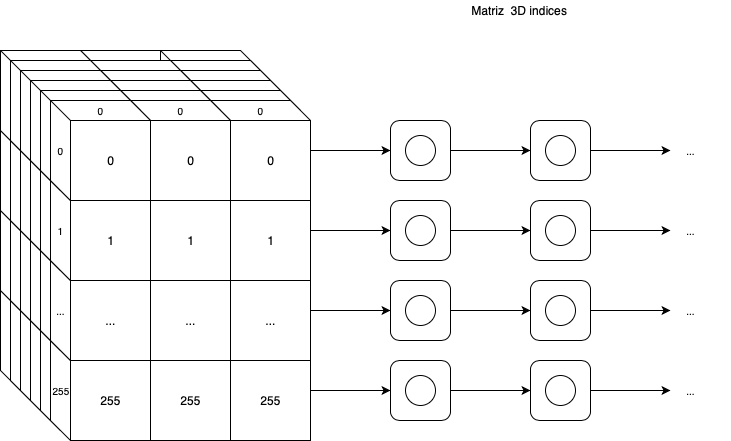
\includegraphics[scale=0.5]{Diagram1.png}}
\caption{Esquema do indice}
\label{fig2}
\end{figure}

Utilizando esta estrutura é possível apenas pesquisar apenas pelos pixels que já se encontram no intervalo de tolerância.  

\section{Explorar vizinhança}

Para explorar a sua volta, cheguei a conclusão que seria extremamente conveniente se, cada uma das minhas estruturas pixéis, também tivesse um conjunto de apontadores para a sua imediata vizinhança e implementei então essa alteração.

\begin{figure}[htbp]
\centerline{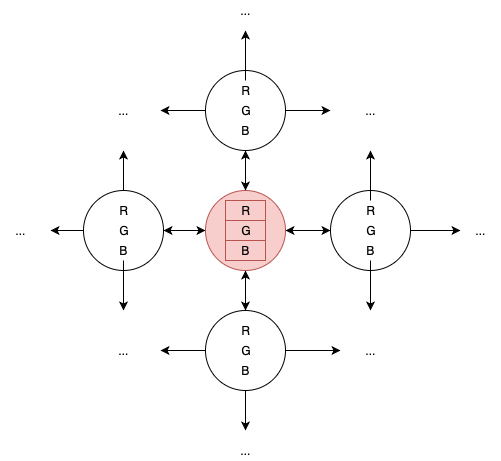
\includegraphics[scale=0.5]{Diagram2.png}}
\caption{Esquema dos pixeís}
\label{fig2}
\end{figure}
 
O algoritmo de exploração consiste então numa função recursiva que, por cada pixel dentro da tolerância visitado, se adiciona à região atualmente a ser explorada e verifica, recursivamente, se os seus vizinhos também devem fazer o mesmo.

\section{Ordenar regiões}

Para ordenar decrescentemente o array de regiões de um determinado frame gerado no passo anterior, utilizei o algoritmo de ordenação quicksort.

\pagebreak
\section{Algumas dificuldades}

Infelizmente, devido a resolução de algumas imagens, o número de chamadas recursivas da função de exploração é extremamente elevado e levava muitas vezes a um overflow do call stack. 

Esta foi sem dúvida a parte da resolução do projeto onde senti mais dificuldade, demorei vários dias sem fazer qualquer progresso e tentei várias soluções para resolver o meu problema, mas não via forma nenhuma de, ou aumentar a memória alocada para o call stack, ou diminuir a memória utilizada no stack, ou até de transformar o meu algoritmo num iterativo. 

\section{Solução do problema}

Gostava imenso da minha solução recursiva, fazia sentido, e eu sabia que funcionava para casos mais pequenos era apenas o call stack que não tinha tamanho suficiente para armazenar todas as chamadas recursivas e os seus correspondentes parâmetros.

Comecei então a pensar se realmente precisaria de utilizar o call stack. Qual a função do call stack neste caso particular para a resolução do meu problema? A sua função resumia-se a manter uma lista funções, ainda por acabar, de exploração de pixéis.

Foi então que me surgiu a ideia, e se, em vez de utilizar os mecanismos de recursividade oferecidos pela linguagem C eu tentasse substituir o meu algoritmo recursivo por um iterativo, mantendo o mesmo algoritmo, mas, implementando a minha própria “recursividade” e, mais importante, a minha própria stack com o tamanho que precisasse?

Esta ideia pareceu me poder gerar alguns problemas: Primeiro, como e que efetuaria uma “chamada recursiva”? Segundo, como é que efetuaria as “execuções” das minhas “chamadas recursivas”?

O primeiro cheguei a conclusão que seria equivalente ao push dos pixéis que pretendo explorar para a stack; O segundo seria equivalente a correr um ciclo tendo primeiro substituindo o pixel a ser explorado pelo pop do valor do pixel no topo da stack até a stack estar vazia.

Desta forma poderia facilmente manter o meu algoritmo que sabia que estava correto fazendo o mínimo de alterações possíveis.

Implementei esta ideia e foi a que utilizei na resolução do meu projeto e que mais tarde ensinei a vários colegas meus com estratégias de solução semelhantes à minha que estavam a ter os mesmos problemas com stack overflows e que não estavam a conseguir resolver o problema.

\section{Resultados obtidos}

O resultado deste projeto foi código extremamente rápido, capaz de pesquisas sucessivas instantâneas de regiões, independentemente da resolução e tamanho do vídeo.

\end{document}